\section{Online Insertion}
Often an interior node pruned as a result of offline symmetry elimination
is required as a start or goal location for an agent.
We handle such cases by inserting back into the graph interior start and goal nodes  
for the duration of the search.
We use the following procedure (highlighted in Figure \ref{fig:insertion}):
\begin{enumerate}
\item{If the start and goal are in the same room no insertion is required.
 Since it is guaranteed that there are no obstacles between the two locations, an optimal 
 path is trivially available. This case will be ignored in the rest of our discussion.}
% take the Manhattan distance between them as the length of the optimal path. }
\item{If the start and goal are not in the same room, connect each of them
to the closest neighbours on each side of the perimeter of the empty room.}
\end{enumerate}
We claim that this procedure retains optimality when searching from the start (or goal) location
to all nodes on the perimeter of its room.

\begin{figure}[t]
	\vspace{-4pt}
       \begin{center}
           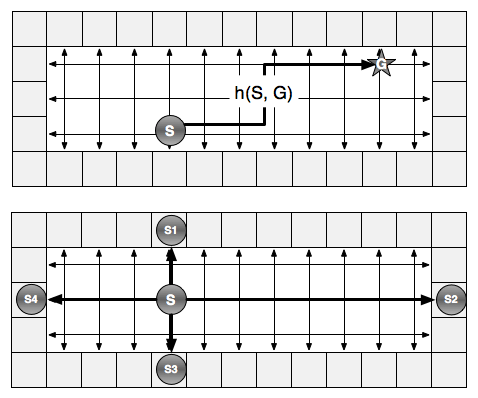
\includegraphics[scale=0.50, trim = 10mm 10mm 10mm 0mm]{diagrams/roomtraversal.png}
       \end{center}
	\vspace{-3pt}
       \caption{(Top) When $m$ and $n$ are in the empty room no insertion is necessary.
				(Bottom) $m$ is a previously pruned interior node.
				We insert $m$ into the graph and connect it to neighbours on each side of the empty room.}
	%\vspace{-15pt}
	\label{fig:insertion}
\end{figure}

\begin{lemma}
\label{thm-insertion}
Let $R$ be an empty rectangular room.
For any nodes $m, n$, with $m$ a re-inserted interior node and $n$ a node on the perimeter,
it is always possible to find an optimal length path which mentions no interior nodes except for $m$.
\end{lemma}
\begin{proof}
We insert $m$ into the graph and connect it to 
$m'_{1}, m'_{2}, m'_{3}, m'_{4}$, the closest neighbours on 
each side of the perimeter.
The weight of each edge incident with $m$ is equal to the Manhattan distance between
$m$ and each $m'_{i}$.
To find an optimal path to $n$ we travel from $m$ to the node $m'_{i}$ which is 
on the same side as $n$ on the perimeter.
From there we travel along the perimeter of $R$ until we reach $n$.
%\par
%Next, suppose $s, g \in N$. 
%In this case we do not insert anything; the length of the optimal path is equal
%to the Manhattan distance between $s$ and $g$.
\end{proof}

Once the search has finished we remove the start and goal from the graph.
The time required in each case (insertion and deletion) is constant.

